% Fignos directives
\renewcommand{\figurename}{FIG}

% Cleveref macros
\providecommand{\crefformat}[2]{}
\providecommand{\Crefformat}[2]{}
\crefformat{figure}{fig.~#2#1#3}
\Crefformat{figure}{Figure~#2#1#3}

% Cleveref fakery
\providecommand{\plusnamesingular}{}
\providecommand{\starnamesingular}{}
\providecommand{\cref}{\plusnamesingular~\ref}
\providecommand{\Cref}{\starnamesingular~\ref}

Some data are shown in
\protect\renewcommand{\plusnamesingular}{fig.}\cref{fig:data}.

\begin{figure}[htbp]
\centering
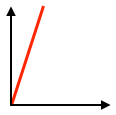
\includegraphics{img/plot1.png}
\caption{Some data.\label{fig:data}}
\end{figure}

\begin{figure}[htbp]
\centering
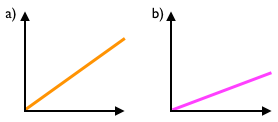
\includegraphics{img/plot2.png}
\caption{More data.\label{fig:more}}
\end{figure}

\protect\renewcommand{\starnamesingular}{Figure}\Cref{fig:more}a and
\protect\renewcommand{\plusnamesingular}{fig.}\cref{fig:more}b give more
data.

\begin{figure}[htbp]
\centering
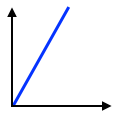
\includegraphics{img/plot3.png}
\caption{Even more
data.\label{fig:0c5b5e21-ec66-491b-9943-ad9192a0f273}}
\end{figure}
